\begin{frame}
\frametitle{Maillage : stratégie de zones}
\vfill
Prise en compte des discontinuités fixes dans le maillage :
\begin{columns}[c]
\column{.5\textwidth}
\begin{itemize}
\item Découpage en \textcolor{blue}{Zones}
\onslide<2->{et \textcolor{red}{Mailles} :}
\begin{align*}
\PbEsp = \textcolor{blue}{\bigcup_{k=1}^K \Adh{\PbEsp_k}}
\onslide<2->{=\textcolor{red}{\bigcup_{i=1}^\NE \Adh{\L_i}} \ ;}
\end{align*}
\item<3-> Maillage :
\begin{align*}
\Mesh = &(\L_i)_{i \in \Range{1}{\NE}} \ ;
\end{align*}
\vfill
\item<3-> Zones physiques données par le modèle CAO ;
\item<3-> Les zones permettront aussi de regrouper les mailles similaires pour appliquer des simplifications dans les calculs.
\end{itemize}
\column{.5\textwidth}
\begin{figure}
	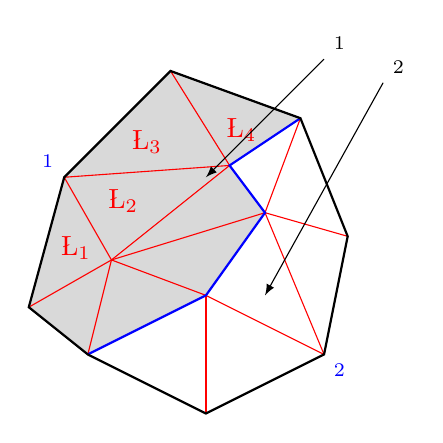
\begin{tikzpicture}[scale=1.5]
\onslide<1->{
\fill[gray!30] (0,0) -- (1,0.5) -- (1.5,1.2) -- (1.2,1.6) -- (1.8,2) -- (0.7,2.4) -- (-0.2,1.5) -- (-0.5,0.4) -- cycle;
}
\onslide<2->{
\draw[-,red] (1,0.5) -- (0.2,0.8);
\draw[-,red] (0,0) -- (0.2,0.8);
\draw[-,red] (-0.5,0.4) -- (0.2,0.8);
\draw[-,red] (-0.2,1.5) -- (0.2,0.8);
\draw[-,red] (-0.2,1.5) -- (1.2,1.6);
\draw[-,red] (0.7,2.4) -- (1.2,1.6);
\draw[-,red] (1.5,1.2) -- (0.2,0.8);
\draw[-,red] (1.2,1.6) -- (0.2,0.8);

\draw[-,red] (1,-0.5) -- (1,0.5);
\draw[-,red] (2,0) -- (1,0.5);
\draw[-,red] (2,0) -- (1.5,1.2);
\draw[-,red] (2.2,1) -- (1.5,1.2);
\draw[-,red] (1.8,2) -- (1.5,1.2);

\draw[red] (-0.1,0.9) node[]{$\L_1$};
\draw[red] (0.3,1.3) node[]{$\L_2$};
\draw[red] (0.5,1.8) node[]{$\L_3$};
\draw[red] (1.3,1.9) node[]{$\L_4$};
}
\onslide<1->{
\draw[-,thick,blue] (0,0) -- (1,0.5) -- (1.5,1.2) -- (1.2,1.6) -- (1.8,2);
\draw[blue] (-0.2,1.5) node[above left]{$\PbEsp_1$};
\draw[blue] (2,0) node[below right]{$\PbEsp_2$};
}
\onslide<1->{
\draw[-,thick] (0,0) -- (1,-0.5) -- (2,0) -- (2.2,1) -- (1.8,2) -- (0.7,2.4) -- (-0.2,1.5) -- (-0.5,0.4) -- cycle;
}
\onslide<1>{
\draw[arrows={latex-}] (1,1.5) -- (2,2.5) node[above right]{$\EPrm_1$};
\draw[arrows={latex-}] (1.5,0.5) -- (2.5,2.3) node[above right]{$\EPrm_2$};
}
	\end{tikzpicture}
\end{figure}
\end{columns}
\vfill
\onslide<3->{
\textcolor{red}{Taille des mailles ? Fonction de la longueur d'onde : «~$\lambda_{\min} / 10$~».}
}
\end{frame}

